% Options for packages loaded elsewhere
\PassOptionsToPackage{unicode}{hyperref}
\PassOptionsToPackage{hyphens}{url}
%
\documentclass[
]{article}
\usepackage{amsmath,amssymb}
\usepackage{lmodern}
\usepackage{iftex}
\ifPDFTeX
  \usepackage[T1]{fontenc}
  \usepackage[utf8]{inputenc}
  \usepackage{textcomp} % provide euro and other symbols
\else % if luatex or xetex
  \usepackage{unicode-math}
  \defaultfontfeatures{Scale=MatchLowercase}
  \defaultfontfeatures[\rmfamily]{Ligatures=TeX,Scale=1}
\fi
% Use upquote if available, for straight quotes in verbatim environments
\IfFileExists{upquote.sty}{\usepackage{upquote}}{}
\IfFileExists{microtype.sty}{% use microtype if available
  \usepackage[]{microtype}
  \UseMicrotypeSet[protrusion]{basicmath} % disable protrusion for tt fonts
}{}
\makeatletter
\@ifundefined{KOMAClassName}{% if non-KOMA class
  \IfFileExists{parskip.sty}{%
    \usepackage{parskip}
  }{% else
    \setlength{\parindent}{0pt}
    \setlength{\parskip}{6pt plus 2pt minus 1pt}}
}{% if KOMA class
  \KOMAoptions{parskip=half}}
\makeatother
\usepackage{xcolor}
\usepackage[margin=1in]{geometry}
\usepackage{color}
\usepackage{fancyvrb}
\newcommand{\VerbBar}{|}
\newcommand{\VERB}{\Verb[commandchars=\\\{\}]}
\DefineVerbatimEnvironment{Highlighting}{Verbatim}{commandchars=\\\{\}}
% Add ',fontsize=\small' for more characters per line
\usepackage{framed}
\definecolor{shadecolor}{RGB}{248,248,248}
\newenvironment{Shaded}{\begin{snugshade}}{\end{snugshade}}
\newcommand{\AlertTok}[1]{\textcolor[rgb]{0.94,0.16,0.16}{#1}}
\newcommand{\AnnotationTok}[1]{\textcolor[rgb]{0.56,0.35,0.01}{\textbf{\textit{#1}}}}
\newcommand{\AttributeTok}[1]{\textcolor[rgb]{0.77,0.63,0.00}{#1}}
\newcommand{\BaseNTok}[1]{\textcolor[rgb]{0.00,0.00,0.81}{#1}}
\newcommand{\BuiltInTok}[1]{#1}
\newcommand{\CharTok}[1]{\textcolor[rgb]{0.31,0.60,0.02}{#1}}
\newcommand{\CommentTok}[1]{\textcolor[rgb]{0.56,0.35,0.01}{\textit{#1}}}
\newcommand{\CommentVarTok}[1]{\textcolor[rgb]{0.56,0.35,0.01}{\textbf{\textit{#1}}}}
\newcommand{\ConstantTok}[1]{\textcolor[rgb]{0.00,0.00,0.00}{#1}}
\newcommand{\ControlFlowTok}[1]{\textcolor[rgb]{0.13,0.29,0.53}{\textbf{#1}}}
\newcommand{\DataTypeTok}[1]{\textcolor[rgb]{0.13,0.29,0.53}{#1}}
\newcommand{\DecValTok}[1]{\textcolor[rgb]{0.00,0.00,0.81}{#1}}
\newcommand{\DocumentationTok}[1]{\textcolor[rgb]{0.56,0.35,0.01}{\textbf{\textit{#1}}}}
\newcommand{\ErrorTok}[1]{\textcolor[rgb]{0.64,0.00,0.00}{\textbf{#1}}}
\newcommand{\ExtensionTok}[1]{#1}
\newcommand{\FloatTok}[1]{\textcolor[rgb]{0.00,0.00,0.81}{#1}}
\newcommand{\FunctionTok}[1]{\textcolor[rgb]{0.00,0.00,0.00}{#1}}
\newcommand{\ImportTok}[1]{#1}
\newcommand{\InformationTok}[1]{\textcolor[rgb]{0.56,0.35,0.01}{\textbf{\textit{#1}}}}
\newcommand{\KeywordTok}[1]{\textcolor[rgb]{0.13,0.29,0.53}{\textbf{#1}}}
\newcommand{\NormalTok}[1]{#1}
\newcommand{\OperatorTok}[1]{\textcolor[rgb]{0.81,0.36,0.00}{\textbf{#1}}}
\newcommand{\OtherTok}[1]{\textcolor[rgb]{0.56,0.35,0.01}{#1}}
\newcommand{\PreprocessorTok}[1]{\textcolor[rgb]{0.56,0.35,0.01}{\textit{#1}}}
\newcommand{\RegionMarkerTok}[1]{#1}
\newcommand{\SpecialCharTok}[1]{\textcolor[rgb]{0.00,0.00,0.00}{#1}}
\newcommand{\SpecialStringTok}[1]{\textcolor[rgb]{0.31,0.60,0.02}{#1}}
\newcommand{\StringTok}[1]{\textcolor[rgb]{0.31,0.60,0.02}{#1}}
\newcommand{\VariableTok}[1]{\textcolor[rgb]{0.00,0.00,0.00}{#1}}
\newcommand{\VerbatimStringTok}[1]{\textcolor[rgb]{0.31,0.60,0.02}{#1}}
\newcommand{\WarningTok}[1]{\textcolor[rgb]{0.56,0.35,0.01}{\textbf{\textit{#1}}}}
\usepackage{graphicx}
\makeatletter
\def\maxwidth{\ifdim\Gin@nat@width>\linewidth\linewidth\else\Gin@nat@width\fi}
\def\maxheight{\ifdim\Gin@nat@height>\textheight\textheight\else\Gin@nat@height\fi}
\makeatother
% Scale images if necessary, so that they will not overflow the page
% margins by default, and it is still possible to overwrite the defaults
% using explicit options in \includegraphics[width, height, ...]{}
\setkeys{Gin}{width=\maxwidth,height=\maxheight,keepaspectratio}
% Set default figure placement to htbp
\makeatletter
\def\fps@figure{htbp}
\makeatother
\setlength{\emergencystretch}{3em} % prevent overfull lines
\providecommand{\tightlist}{%
  \setlength{\itemsep}{0pt}\setlength{\parskip}{0pt}}
\setcounter{secnumdepth}{-\maxdimen} % remove section numbering
\ifLuaTeX
  \usepackage{selnolig}  % disable illegal ligatures
\fi
\IfFileExists{bookmark.sty}{\usepackage{bookmark}}{\usepackage{hyperref}}
\IfFileExists{xurl.sty}{\usepackage{xurl}}{} % add URL line breaks if available
\urlstyle{same} % disable monospaced font for URLs
\hypersetup{
  pdftitle={WORKING EXAMPLE 1},
  pdfauthor={Itziar Irigoien, Patricia Mas-Bermejo, Sergi Papiol, Neus Barrantes-Vidal,; Araceli Rosa, and Concepción Arenas},
  hidelinks,
  pdfcreator={LaTeX via pandoc}}

\title{WORKING EXAMPLE 1}
\usepackage{etoolbox}
\makeatletter
\providecommand{\subtitle}[1]{% add subtitle to \maketitle
  \apptocmd{\@title}{\par {\large #1 \par}}{}{}
}
\makeatother
\subtitle{In: A guide to test association between Polygenic Risk Scores
and psychological and psychiatric traits: practical examples}
\author{Itziar Irigoien, Patricia Mas-Bermejo, Sergi Papiol, Neus
Barrantes-Vidal, \and Araceli Rosa, and Concepción Arenas}
\date{}

\begin{document}
\maketitle

\hypertarget{working-flow-and-code}{%
\subsection{Working flow and code}\label{working-flow-and-code}}

In this example we simulate 9 PRSs, and a continuous trait, with sex,
clinical diagnosis (with 2 categories), age, and two Principal
Components as covariates.

\begin{itemize}
\tightlist
\item
  data reading
\end{itemize}

\begin{Shaded}
\begin{Highlighting}[]
\NormalTok{dat }\OtherTok{\textless{}{-}} \FunctionTok{read.table}\NormalTok{(}\StringTok{"WExample1.csv"}\NormalTok{, }\AttributeTok{header=}\ConstantTok{TRUE}\NormalTok{, }\AttributeTok{sep=}\StringTok{";"}\NormalTok{, }\AttributeTok{dec=}\StringTok{","}\NormalTok{)}
\FunctionTok{names}\NormalTok{(dat) }\CommentTok{\#}
\end{Highlighting}
\end{Shaded}

\begin{verbatim}
##  [1] "Sex"        "Diagnostic" "Age"        "Trait"      "PRS.1"     
##  [6] "PRS.2"      "PRS.3"      "PRS.4"      "PRS.5"      "PRS.6"     
## [11] "PRS.7"      "PRS.8"      "PRS.9"      "PC1"        "PC2"
\end{verbatim}

\bigskip

\begin{itemize}
\tightlist
\item
  do not forget to declare the categorical variables as factors
\end{itemize}

\begin{Shaded}
\begin{Highlighting}[]
\NormalTok{dat}\SpecialCharTok{$}\NormalTok{Sex }\OtherTok{\textless{}{-}} \FunctionTok{as.factor}\NormalTok{(dat}\SpecialCharTok{$}\NormalTok{Sex)}
\NormalTok{dat}\SpecialCharTok{$}\NormalTok{Diagnostic }\OtherTok{\textless{}{-}} \FunctionTok{as.factor}\NormalTok{(dat}\SpecialCharTok{$}\NormalTok{Diagnostic)}
\end{Highlighting}
\end{Shaded}

\hypertarget{what-full-model-should-be-considered}{%
\subsection{1. What full model should be
considered?}\label{what-full-model-should-be-considered}}

First, given a particular PRS (named PRS.i), consider all the possible
full models:

\begin{itemize}
\tightlist
\item
  FM\(_{WI}\): Trait versus PRS.i + Sex + Diagnostic + Age + PC1 + PC2
\item
  FM\(_{Sex}\): Trait versus PRS.i + Sex + PRS.i · Sex + Diagnostic +
  Age + PC1 + PC2
\item
  FM\(_{Diagnostic}\): Trait versus PRS.i + Sex + Diagnostic + PRS.i ·
  Diagnostic + Age + PC1 + PC2
\item
  FM\(_{Sex/Diagnostic}\): Trait versus PRS.i + Sex + PRS.i · Sex +
  Diagnostic + PRS.i · Diagnostic + Age + PC1 + PC2
\end{itemize}

\hypertarget{how-to-make-a-prs-ranking-to-find-the-important-ones}{%
\subsection{2. How to make a PRS ranking to find the important
ones?}\label{how-to-make-a-prs-ranking-to-find-the-important-ones}}

As is described in the paper, for each model, calculate the coefficient
of determination \(R^2\) and calculate the sum:
\(S = R^2_{WI} + R^2_{Sex} + R^2_{Diagnostic} + R^2_{Sex/Diagnostic}\).

According to S, list the PRSs in decreasing order:

\begin{Shaded}
\begin{Highlighting}[]
\NormalTok{out }\OtherTok{\textless{}{-}} \FunctionTok{orderR2}\NormalTok{(dat, }\AttributeTok{yname=}\StringTok{"Trait"}\NormalTok{, }\AttributeTok{prsname =} \StringTok{"PRS."}\NormalTok{)}
\FunctionTok{head}\NormalTok{(out)}
\end{Highlighting}
\end{Shaded}

\begin{verbatim}
##           Model1     Model2     Model3     Model4       Sum
## PRS.4 0.06561329 0.07420427 0.12600084 0.15146070 0.4172791
## PRS.6 0.05596966 0.06220536 0.13638253 0.15759204 0.4121496
## PRS.2 0.04973955 0.05309214 0.11850006 0.12356753 0.3448993
## PRS.5 0.05308815 0.06728312 0.10264612 0.11770778 0.3407252
## PRS.8 0.07995274 0.08034903 0.08088220 0.08141782 0.3226018
## PRS.9 0.07932875 0.08028067 0.07933969 0.08030066 0.3192498
\end{verbatim}

\begin{Shaded}
\begin{Highlighting}[]
\FunctionTok{write.csv2}\NormalTok{(out,}\AttributeTok{file=}\StringTok{"WExample1\_Ordered\_PRS.csv"}\NormalTok{)}
\end{Highlighting}
\end{Shaded}

\bigskip

Plot the sum of coefficients of determination \(S_{R^2}\). Lines: in
blue the median; in black the mean

\begin{Shaded}
\begin{Highlighting}[]
\NormalTok{out }\OtherTok{\textless{}{-}} \FunctionTok{data.frame}\NormalTok{(out) }
\NormalTok{nPRS }\OtherTok{\textless{}{-}} \FunctionTok{dim}\NormalTok{(out)[}\DecValTok{1}\NormalTok{]}
\NormalTok{select }\OtherTok{\textless{}{-}} \FunctionTok{grep}\NormalTok{(}\StringTok{"Model"}\NormalTok{, }\FunctionTok{names}\NormalTok{(out), }\AttributeTok{value=}\ConstantTok{FALSE}\NormalTok{)}
\NormalTok{out}\SpecialCharTok{$}\NormalTok{effect }\OtherTok{\textless{}{-}}\NormalTok{ out}\SpecialCharTok{$}\NormalTok{Sum}
\NormalTok{sds }\OtherTok{\textless{}{-}} \FunctionTok{apply}\NormalTok{(out[, select], }\DecValTok{1}\NormalTok{, sd)}
\NormalTok{out}\SpecialCharTok{$}\NormalTok{lower }\OtherTok{\textless{}{-}}\NormalTok{ out}\SpecialCharTok{$}\NormalTok{effect }\SpecialCharTok{{-}}\NormalTok{ sds}
\NormalTok{out}\SpecialCharTok{$}\NormalTok{upper }\OtherTok{\textless{}{-}}\NormalTok{ out}\SpecialCharTok{$}\NormalTok{effect }\SpecialCharTok{+}\NormalTok{ sds}
\NormalTok{out}\SpecialCharTok{$}\NormalTok{rank }\OtherTok{\textless{}{-}}\NormalTok{ nPRS}\SpecialCharTok{:}\DecValTok{1}

\NormalTok{n }\OtherTok{\textless{}{-}} \FunctionTok{dim}\NormalTok{(out)[}\DecValTok{1}\NormalTok{]}
\FunctionTok{ggplot}\NormalTok{(}\AttributeTok{data=}\NormalTok{out, }\FunctionTok{aes}\NormalTok{(}\AttributeTok{y=}\NormalTok{rank, }\AttributeTok{x=}\NormalTok{effect, }\AttributeTok{xmin=}\NormalTok{lower, }\AttributeTok{xmax=}\NormalTok{upper)) }\SpecialCharTok{+}
  \FunctionTok{geom\_point}\NormalTok{() }\SpecialCharTok{+}
  \FunctionTok{geom\_errorbarh}\NormalTok{(}\AttributeTok{height=}\NormalTok{.}\DecValTok{1}\NormalTok{) }\SpecialCharTok{+}
  \FunctionTok{scale\_y\_continuous}\NormalTok{(}\AttributeTok{name=}\ConstantTok{NULL}\NormalTok{, }\AttributeTok{breaks=}\NormalTok{ n}\SpecialCharTok{:}\DecValTok{1}\NormalTok{, }\AttributeTok{labels=}\FunctionTok{row.names}\NormalTok{(out), }\AttributeTok{position=}\StringTok{"right"}\NormalTok{) }\SpecialCharTok{+}
  \FunctionTok{labs}\NormalTok{(}\AttributeTok{title=}\StringTok{\textquotesingle{}\textquotesingle{}}\NormalTok{, }\AttributeTok{x=}\StringTok{\textquotesingle{}Sum R\^{}2\textquotesingle{}}\NormalTok{, }\AttributeTok{y =} \StringTok{\textquotesingle{}PRS\textquotesingle{}}\NormalTok{) }\SpecialCharTok{+}
  \FunctionTok{geom\_vline}\NormalTok{(}\AttributeTok{xintercept=}\FunctionTok{mean}\NormalTok{(out}\SpecialCharTok{$}\NormalTok{effect), }\AttributeTok{color=}\StringTok{\textquotesingle{}black\textquotesingle{}}\NormalTok{, }\AttributeTok{linetype=}\StringTok{\textquotesingle{}dashed\textquotesingle{}}\NormalTok{) }\SpecialCharTok{+}
  \FunctionTok{geom\_vline}\NormalTok{(}\AttributeTok{xintercept=}\FunctionTok{median}\NormalTok{(out}\SpecialCharTok{$}\NormalTok{effect), }\AttributeTok{color=}\StringTok{\textquotesingle{}blue\textquotesingle{}}\NormalTok{, }\AttributeTok{linetype=}\StringTok{\textquotesingle{}dashed\textquotesingle{}}\NormalTok{) }\SpecialCharTok{+}
  \FunctionTok{theme\_minimal}\NormalTok{()}
\end{Highlighting}
\end{Shaded}

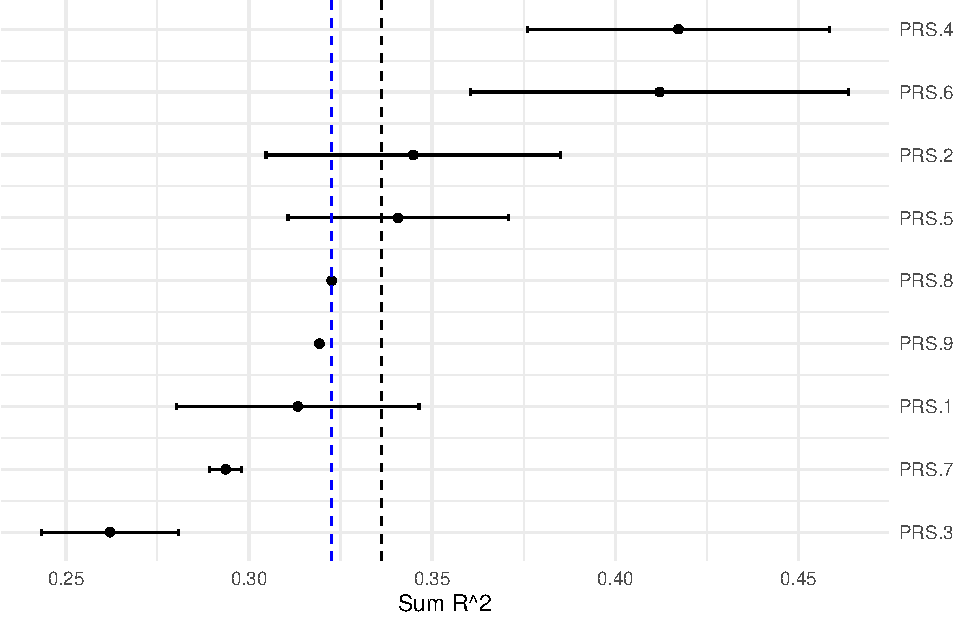
\includegraphics{WorkingExample1_code_files/figure-latex/unnamed-chunk-5-1.pdf}

According to the obtained results, first, PRS.4 is selected to analyse
its possible association with the Trait.

\hypertarget{which-model-of-all-the-possible-ones-should-be-used}{%
\subsection{3. Which model, of all the possible ones, should be
used?}\label{which-model-of-all-the-possible-ones-should-be-used}}

The following Figure represents the scatter plot of Trait versus PRS.4
separated by Sex and Diagnostic groups.

\begin{Shaded}
\begin{Highlighting}[]
\CommentTok{\# First candidate PRS.4}
\CommentTok{\# Plot it}
\FunctionTok{ggplot}\NormalTok{(dat, }\FunctionTok{aes}\NormalTok{(}\AttributeTok{x=}\NormalTok{PRS}\FloatTok{.4}\NormalTok{, }\AttributeTok{y=}\NormalTok{Trait)) }\SpecialCharTok{+}
  \FunctionTok{geom\_point}\NormalTok{() }\SpecialCharTok{+}
  \FunctionTok{geom\_smooth}\NormalTok{(}\AttributeTok{method=}\NormalTok{lm, }\AttributeTok{se=}\ConstantTok{FALSE}\NormalTok{)}\SpecialCharTok{+}
  \FunctionTok{facet\_grid}\NormalTok{(Sex }\SpecialCharTok{\textasciitilde{}}\NormalTok{ Diagnostic, }\AttributeTok{labeller=}\NormalTok{label\_both)}
\end{Highlighting}
\end{Shaded}

\begin{verbatim}
## `geom_smooth()` using formula = 'y ~ x'
\end{verbatim}

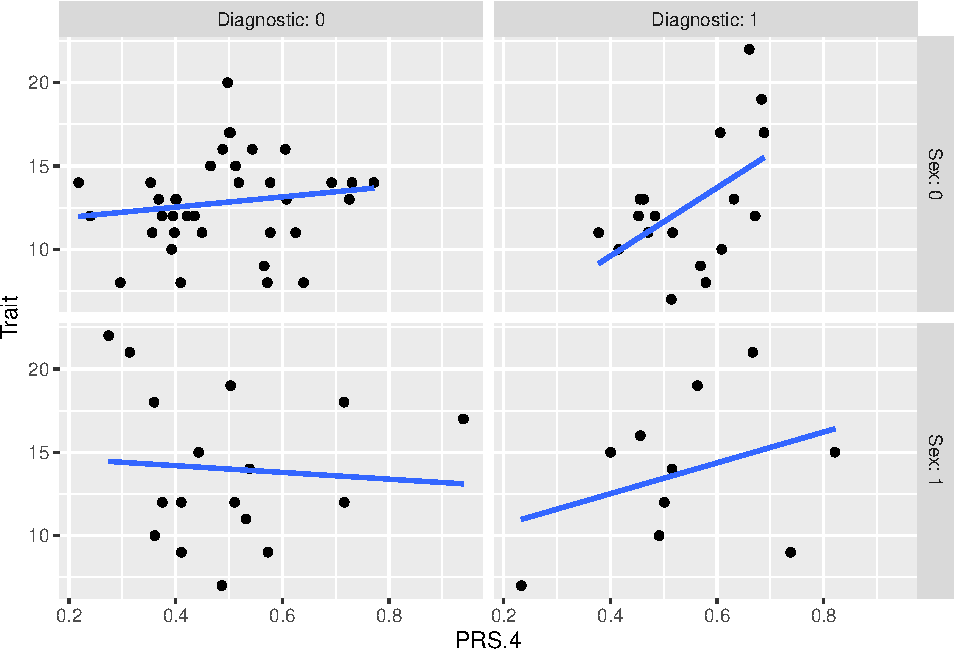
\includegraphics{WorkingExample1_code_files/figure-latex/unnamed-chunk-6-1.pdf}

Observing the slopes of the lines, it seems that a different
relationship between Trait and PRS.4 could be expected depending on the
diagnostic group, but not depending on the sex group.Thus, we set the
full model candidate (FM):
\(Trait \sim PRS + Sex + Diagnostic + PRS\cdot Diagnostic + PC1 +PC2\).

\hypertarget{for-a-continuous-trait-what-steps-should-be-followed-for-a-correct-analysis}{%
\subsection{4. For a continuous trait, what steps should be followed for
a correct
analysis?}\label{for-a-continuous-trait-what-steps-should-be-followed-for-a-correct-analysis}}

\begin{itemize}
\tightlist
\item
  \textbf{4.1. How is the candidate model validated?}
\end{itemize}

First, we validate the normality of the errors and the constant variance
conditions (see the figures and the results of Shapiro test and Levene
test.

\begin{Shaded}
\begin{Highlighting}[]
\CommentTok{\#model}
\NormalTok{FM }\OtherTok{\textless{}{-}} \FunctionTok{lm}\NormalTok{(Trait }\SpecialCharTok{\textasciitilde{}}\NormalTok{ PRS}\FloatTok{.4}\SpecialCharTok{*}\NormalTok{Diagnostic }\SpecialCharTok{+}\NormalTok{ Sex }\SpecialCharTok{+}\NormalTok{ Age }\SpecialCharTok{+}\NormalTok{ PC1 }\SpecialCharTok{+}\NormalTok{ PC2, }\AttributeTok{data=}\NormalTok{dat)}
\CommentTok{\#qq{-}plot for normality }
\FunctionTok{plot}\NormalTok{(FM,}\DecValTok{2}\NormalTok{)   }
\end{Highlighting}
\end{Shaded}

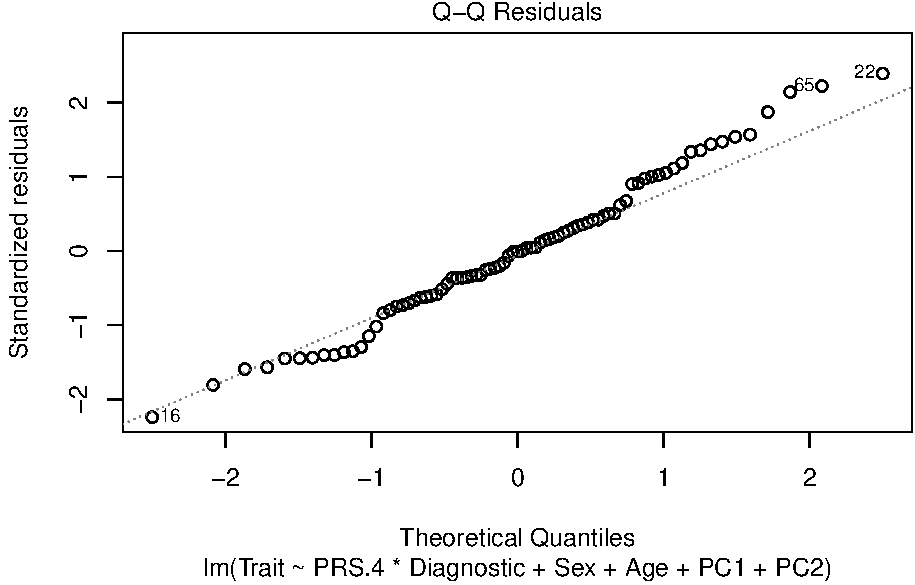
\includegraphics{WorkingExample1_code_files/figure-latex/unnamed-chunk-7-1.pdf}

\begin{Shaded}
\begin{Highlighting}[]
\CommentTok{\#Shapiro{-}Wilk test}
\FunctionTok{shapiro.test}\NormalTok{(FM}\SpecialCharTok{$}\NormalTok{residuals)}
\end{Highlighting}
\end{Shaded}

\begin{verbatim}
## 
##  Shapiro-Wilk normality test
## 
## data:  FM$residuals
## W = 0.98413, p-value = 0.4166
\end{verbatim}

\begin{Shaded}
\begin{Highlighting}[]
\CommentTok{\#plot for variances}
\NormalTok{d }\OtherTok{\textless{}{-}} \FunctionTok{fortify}\NormalTok{(FM)}
\FunctionTok{ggplot}\NormalTok{(d,}\FunctionTok{aes}\NormalTok{(}\AttributeTok{x=}\NormalTok{.fitted, }\AttributeTok{y=}\NormalTok{.stdresid, }\AttributeTok{colour=}\NormalTok{Diagnostic)) }\SpecialCharTok{+} 
  \FunctionTok{geom\_point}\NormalTok{() }\SpecialCharTok{+} 
  \FunctionTok{geom\_hline}\NormalTok{(}\AttributeTok{yintercept=}\DecValTok{0}\NormalTok{, }\AttributeTok{col=}\StringTok{"red"}\NormalTok{) }\SpecialCharTok{+}
  \FunctionTok{facet\_wrap}\NormalTok{(.}\SpecialCharTok{\textasciitilde{}}\NormalTok{Diagnostic)}
\end{Highlighting}
\end{Shaded}

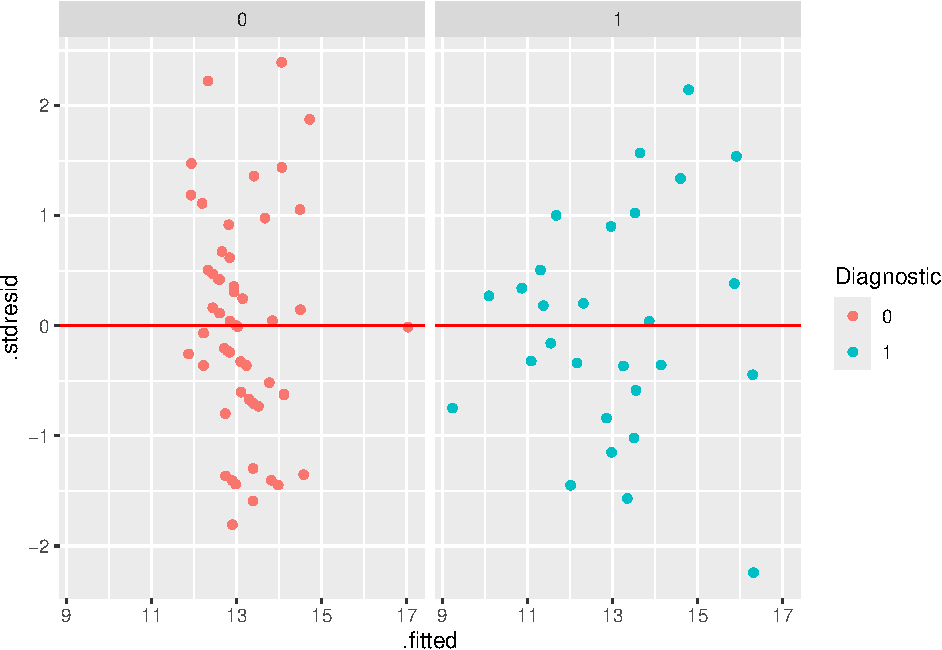
\includegraphics{WorkingExample1_code_files/figure-latex/unnamed-chunk-9-1.pdf}

\begin{Shaded}
\begin{Highlighting}[]
\CommentTok{\#Levene\textquotesingle{}s test}
\FunctionTok{leveneTest}\NormalTok{(.stdresid }\SpecialCharTok{\textasciitilde{}}\NormalTok{ Diagnostic, }\AttributeTok{data=}\NormalTok{d)}
\end{Highlighting}
\end{Shaded}

\begin{verbatim}
## Levene's Test for Homogeneity of Variance (center = median)
##       Df F value Pr(>F)
## group  1  0.1193 0.7307
##       79
\end{verbatim}

\bigskip

Having the full model validated, we can use it.

\begin{itemize}
\tightlist
\item
  \textbf{4.3 How a possible association is established?}
\end{itemize}

\begin{Shaded}
\begin{Highlighting}[]
\FunctionTok{summary}\NormalTok{(FM)}
\end{Highlighting}
\end{Shaded}

\begin{verbatim}
## 
## Call:
## lm(formula = Trait ~ PRS.4 * Diagnostic + Sex + Age + PC1 + PC2, 
##     data = dat)
## 
## Residuals:
##     Min      1Q  Median      3Q     Max 
## -7.3117 -2.1180 -0.0277  1.6987  7.9418 
## 
## Coefficients:
##                   Estimate Std. Error t value Pr(>|t|)    
## (Intercept)       14.81613    2.80605   5.280 1.28e-06 ***
## PRS.4             -1.04058    3.71031  -0.280   0.7799    
## Diagnostic1       -8.32066    3.62154  -2.298   0.0245 *  
## Sex1               1.29952    0.83922   1.548   0.1258    
## Age               -0.07070    0.08635  -0.819   0.4156    
## PC1                0.92650    6.45497   0.144   0.8863    
## PC2                8.03272    6.22984   1.289   0.2013    
## PRS.4:Diagnostic1 15.02560    6.69040   2.246   0.0277 *  
## ---
## Signif. codes:  0 '***' 0.001 '**' 0.01 '*' 0.05 '.' 0.1 ' ' 1
## 
## Residual standard error: 3.541 on 73 degrees of freedom
## Multiple R-squared:  0.126,  Adjusted R-squared:  0.04219 
## F-statistic: 1.503 on 7 and 73 DF,  p-value: 0.1796
\end{verbatim}

Next table shows the parameters and hypothesis (columns 1-3), together
with the standard output for this type of analysis (columns 4-7). This
output allows the model equation to be built and it would be used if the
objective of the study is to predict the Trait values.

\begin{table}[h!]
\centering
\begin{tabular}{l|ccrrrr}
\hline
              &  Parameter & Null Hypothesis & Estimate & Std. Error & t value & $p$-value\\
\hline
Intercept & $b_0$ &  $b_0=0$ & 14.816 & 2.806 &  5.280 & 1.28e-06\\
PRS.4 & $b_1$ &  $b_1=0$ & -1.041 & 3.710 & -0.280 &  0.780\\
Diagnostic1 & $b_2$ &  $b_2=0$ & -8.321 & 3.622 & -2.298 &  0.025\\
Sex1 & $b_3$ &  $b_3=0$ & 1.300 & 0.839 &  1.548 &  0.126\\
Age & $b_4$ &  $b_4=0$ & -0.071 & 0.086 & -0.819 &  0.416\\
PC1 & $b_5$ &  $b_5=0$ & 0.927 & 6.455 &  0.144 &  0.886\\ 
PC2 & $b_6$ &  $b_6=0$ & 8.033 & 6.230 &  1.289 &  0.201\\
PRS.4:Diagnostic1 & $b_7$ &  $b_7=0$ & 15.026 & 6.690 &  2.246 &  0.028\\
 \hline
\end{tabular}
\caption{\label{tab:Table2}: Working example 1. Parameters, null hypothesis, estimates, standard errors, $t$ statistics, and $p$-values for the regression coefficients in the FM$_{Diagnostic}$.}
\end{table}

\bigskip

The PRS.4 coefficient will vary depending on the diagnostic group each
individual belongs to, being:

\begin{itemize}
\tightlist
\item
  if Diagnostic = 0,
  \(\widehat{Trait} = 14.816 + -1.041\, PRS.4 + 1.3\,Sex -0.071\,Age + 0.927\,PC1 + 8.033\,PC2\)
\item
  if Diagnostic = 1,
  \(\widehat{Trait} = (14.816 -8.321) + (-1.041+15.022)\,PRS.4 + 1.3\,Sex -0.071\,Age + 0.927\,PC1 + 8.033\,PC2\)
\end{itemize}

where Sex takes values 0 or 1, depending on whether the individual under
study is male or female, affecting only the value of the intercept.

However, if the objective is to evaluate the possible association
between Trait and PRS.4, it can be interesting to check whether the
respective PRS.4 coefficients under each Diagnostic group are
considerable or not. Note that these coefficients vary according to the
Diagnosis group being \(b_1\) for the Diagnostic group 0, which has been
taken as the basal group; \(b_1 + b_7\) for the Diagnostic 1:

\begin{Shaded}
\begin{Highlighting}[]
\FunctionTok{summary}\NormalTok{(}\FunctionTok{glht}\NormalTok{(FM, }\StringTok{"PRS.4 = 0"}\NormalTok{))}
\end{Highlighting}
\end{Shaded}

\begin{verbatim}
## 
##   Simultaneous Tests for General Linear Hypotheses
## 
## Fit: lm(formula = Trait ~ PRS.4 * Diagnostic + Sex + Age + PC1 + PC2, 
##     data = dat)
## 
## Linear Hypotheses:
##            Estimate Std. Error t value Pr(>|t|)
## PRS.4 == 0   -1.041      3.710   -0.28     0.78
## (Adjusted p values reported -- single-step method)
\end{verbatim}

\begin{Shaded}
\begin{Highlighting}[]
\FunctionTok{summary}\NormalTok{(}\FunctionTok{glht}\NormalTok{(FM, }\StringTok{"PRS.4  + PRS.4:Diagnostic1 = 0"}\NormalTok{))}
\end{Highlighting}
\end{Shaded}

\begin{verbatim}
## 
##   Simultaneous Tests for General Linear Hypotheses
## 
## Fit: lm(formula = Trait ~ PRS.4 * Diagnostic + Sex + Age + PC1 + PC2, 
##     data = dat)
## 
## Linear Hypotheses:
##                                Estimate Std. Error t value Pr(>|t|)  
## PRS.4 + PRS.4:Diagnostic1 == 0    13.98       5.55    2.52   0.0139 *
## ---
## Signif. codes:  0 '***' 0.001 '**' 0.01 '*' 0.05 '.' 0.1 ' ' 1
## (Adjusted p values reported -- single-step method)
\end{verbatim}

That means that for Diagnostic group 0 there is no relevant association
(coeff = -1.041), but for Diagnostic group 1, the association is strong,
positive (coeff = 13.980), and significant (p-value = 0.014).

-\textbf{Last step: We move to the next PRS.}

\end{document}
